\section{Failure diagnosis and recovery}
\label{chapter:05}

% block-id: auto.05.p1
\hypertarget{auto.05.p1}{}
The failure-diagnosis case retains an actual unit-conversion API error and its repair. A transport response from an MCP call does not by itself establish successful application execution: a tool may return an error as an ordinary string while the protocol-level isError flag remains false. Diagnosis therefore examines the returned content, exception context, and expected result structure, corrects the API invocation, and checks the successful response and subsequent solver outputs in a new run.

% block-id: auto.05.p2
\hypertarget{auto.05.p2}{}
The repair preserves the original physical parameters and constraints. The failed call, revised call, and linked Maxwell result form a comparison that identifies the interface layer as the site of repair. The protocol report establishes whether the tool performed the intended operation; the physical report remains responsible for port and power acceptance. Run identities connect the two reports.

% block-id: auto.05.p3
\hypertarget{auto.05.p3}{}
The A–φ case illustrates a different diagnostic task. The executor reads existing field, potential, and derivative diagnostics and records completed execution while retaining the failed\_retained\_phi\_gauge physical status. Changes to sampling or display parameters alter how the saved field is observed. The original field inputs, sample positions, diagnostic formulas, and acceptance thresholds jointly support interpretation; subsequent repair must address the numerical treatment of potential and gauge conditions. \cite{FEMDOC}

% block-id: auto.05.figure
\hypertarget{auto.05.figure}{}
\begin{figure}[!htbp]
\centering
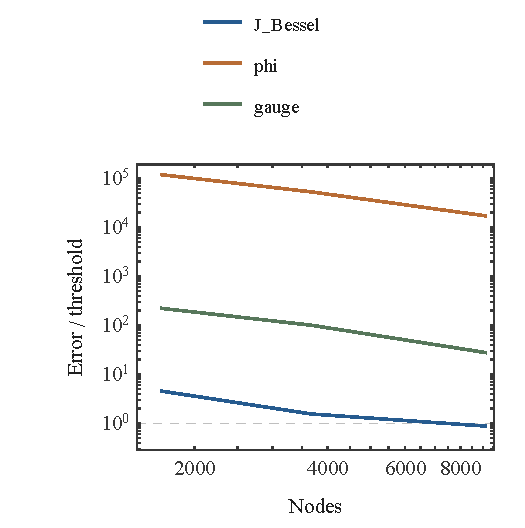
\includegraphics[width=\linewidth,height=.72\textheight,keepaspectratio]{../../assets/en/aphi_gates.pdf}
\caption{A–φ cylinder calibration metrics. Three grids and their metric targets are shown separately. The three cylinder levels contain 1683, 3672, and 9108 nodes. Errors are normalized by their respective acceptance targets, with the horizontal line indicating a unit ratio.}
\label{fig:aphi_gates}
\end{figure}

% block-id: auto.05.p4
\hypertarget{auto.05.p4}{}
The Wolfram tool record also includes process cleanup after frontend work completed: a save receipt was observed, the owned helper process ultimately exited with code 137, and the cleanup reason was retained separately. Interpreting such a run requires the completion receipt, saved outputs, and process-termination reason together. One exit code cannot fully describe work spanning a frontend and kernel.

% block-id: auto.05.p5
\hypertarget{auto.05.p5}{}
Together, the six archived rc.2 case classes cover calibration and Notebook production, native model construction and solution, cross-solver comparison, source extension, interface repair, and interpretation of numerical failure. Their common outputs are identifiable inputs, source, calls, results, and acceptance explanations. A successor can reproduce a problem at the relevant layer and continue the investigation under a new run identity.
